\chapter{Spektrales Lernen auf Graphen}
\label{spektrales_lernen}

Das spektrale Lernen auf Graphen \bzw{} die Formulierung eines spektralen Faltungsoperator auf Graphen basiert auf der spektralen Graphentheorie, \dhe{} der Betrachtung des Spektrums eines Graphen definiert über dessen Eigenwerte.
Merkmale auf den Knoten eines Graphen können über das Spektrum analog zur Fourier-Transformation in dessen Frequenzraum zerlegt und wieder retransformiert werden.
Diese Transformation erlaubt damit die fundamentale Formulierung eines Faltungsoperators in der spektralen Domäne des Graphen.
Da der so definierte spektrale Faltungsoperator insbesondere rotationsinvariant ist, wird dieser im Verlauf des Kapitels für den Kontext von Graphen im euklidschen Raum modifiziert.

Durch die spektrale Formulierung kann weiterhin ein effizientes Pooling auf Graphen formuliert werden, welches uns erlaubt, Netzarchitekturen auf Graphen völlig analog zu klassischen \glspl{CNN} auf zweidimensionalen Bildern zu generieren.

\section{Spektrale Graphentheorie}
\label{spektrale_graphentheorie}

Es gibt 2 große Quellen hier:
\begin{itemize}
  \item Spectral Graph Theory by Chung
  \item Discrete Laplace-Beltrami Operator
\end{itemize}
+ 5 zum Lernen:
\begin{itemize}
  \item Semi Supervised Classification
  \item Fast Localized Spectral Filterung
  \item Wavelets on Graphs via Spectral Graph Theory
  \item The Emerging Field of Signal Processing on Graphs
  \item How powerful are Graph Convolutions? (Review)
\end{itemize}

\subsection{Eigenwerte und Eigenvektoren reell symmetrischer Matrizen}
\label{eigenwerte_symmetrischer_matrizen}

\todo{intro}

$\ma{M} \in \gls{R}^{N \times N}$.
$\gls{eiv} \in \gls{R}^{N}$, $\gls{eiv} \neq \mathbf{0}$.
$\gls{lambda} \in \gls{R}$.
\emph{Eigenwertproblem} $\ma{M}\gls{eiv} = \gls{lambda}\gls{eiv}$.
Zu einem \emph{Eigenwert} $\gls{lambda}$ gibt es unendlich viele (skalierte) \emph{Eigenvektoren} \gls{eiv}.
Wir definieren den Eigenvektor \gls{eiv} eines Eigenwertes \gls{lambda} daher eindeutig über die Bedingung $\left\|\gls{eiv}\right\|_2 = 1$.
Sei \ma{M} weiterhin symmetrisch, \dhe{} $\ma{M} = \ma{M}^{\top}$.
Dann gilt für zwei unterschiedliche Eigenvektoren $\gls{eiv}_1$ und $\gls{eiv}_2$, dass $\gls{eiv}_1 \gls{ortho} \gls{eiv}_2$.
Weiterhin hat \ma{M} genau $N$ reelle Eigenwerte mit ${\left\{\gls{lambda}_i\right\}}_{i=1}^N$.

Wir definieren zu \ma{M} die orthogonale \emph{Eigenvektormatrix} $\gls{Eiv} = \left[\gls{eiv}_1, \ldots, \gls{eiv}_n\right] \in \gls{R}^{N \times N}$, wobei $\gls{Eiv}\gls{Eiv}^{\top}=\gls{I}$, und dessen korrespondierende Eigenwertdiagonalmatrix $\gls{Lambda} = \gls{diag}\left(\left[\gls{lambda}_1, \ldots, \gls{lambda}_N\right]\right)$, \dhe{} $\gls{Lambda}_{ii} = \gls{lambda}_i$.
Dann gilt $\ma{M}\gls{Eiv} = \gls{Eiv}\gls{Lambda}$ und insbesondere ist \ma{M} diagonalisierbar über
\begin{equation}
  \ma{M} = \ma{M}\gls{Eiv}\gls{Eiv}^{\top} = \gls{Eiv}\gls{Lambda}\gls{Eiv}^{\top}.
\end{equation}

Weiterhin gilt für die $k$te Potenz von $\ma{M}$, $k \in \gls{N}$,
\begin{equation}
  \ma{M}^k = {\left(\gls{Eiv}\gls{Lambda}\gls{Eiv}^{\top}\right)}^k = \gls{Eiv}\gls{Lambda}^k\gls{Eiv}^{\top}.
\end{equation}

Dieser Zusammenhang lässt sich verdeutlichen, wenn man die Potenz ausschreibt:
\begin{equation*}
  {\left(\gls{Eiv}\gls{Lambda}\gls{Eiv}^{\top}\right)}^k = \gls{Eiv}\gls{Lambda}\gls{Eiv}^{\top}\gls{Eiv}\gls{Lambda}\gls{Eiv}^{\top}\prod^{k-2}_{i=1} \gls{Eiv}\gls{Lambda}\gls{Eiv}^{\top} = \gls{Eiv}\gls{Lambda}^2\gls{Eiv}^{\top} \prod^{k-2}_{i=1} \gls{Eiv}\gls{Lambda}\gls{Eiv}^{\top} = \gls{Eiv}\gls{Lambda}^k \gls{Eiv}^{\top}.
\end{equation*}

Falls \ma{M} weiterhin \emph{schwach diagonaldominant} ist, \dhe{}
\begin{equation}
  \sum_{\substack{j=1\\j \neq i}}^N \left|\ma{M}_{ij}\right| \leq \left|\ma{M}\right|_{ii},
  \label{eq:schwach_diagonaldominant}
\end{equation}
und $\ma{M}_{ii} \geq 0$ für alle $i \in \left\{1, \ldots, N\right\}$, ist \ma{M} \emph{positiv semidefinit}, \dhe{} $\ve{x}^{\top}\ma{M}\ve{x} \geq 0$ für alle $\ve{x} \in \gls{R}^{N}$.
Eigenwerte symmetrischer positiv semidefiniter Matrizen $\lambda_i \in \gls{R+}$ sind positiv reell und es lässt sich folglich auf diesen eine Ordnung definieren mit $0 \leq \gls{lambda}_1 \leq \cdots \leq \gls{lambda}_N \coloneqq \gls{lambdamax}$.

\todo{quelle}

\subsection{Laplace-Matrix}
\label{laplace_matrix}

Our eigenvalues relate well to other graph invariants for general graphs in a way that other definitions (such as the eigenvalues of adjacency matrices) often fail to do.
The advantages of this definition are perhaps due to the fact that it is consistent with the eigenvalues in spectral geometry and in stochastic processes.
Many results which were only known for regular graphs can be generalized to all graphs~\cite{Chung}.

\todo{intro}

Für einen schleifenlosen, ungerichteteten, gewichtet oder ungewichteten Graphen \gls{G} und dessen Adjazenzmatrix \gls{A} mit Gradmatrix \gls{D} ist die \emph{kombinatorische Laplace-Matrix} \gls{L} definiert als $\gls{L} = \gls{D} - \gls{A}$~\cite{Chung}.
Die \emph{normalisierte Laplace-Matrix} \gls{Lnorm} ist definiert als $\gls{Lnorm} = \gls{D}^{-\frac{1}{2}} \gls{L} \gls{D}^{-\frac{1}{2}}$ mit der Konvention, dass $\gls{D}^{-\frac{1}{2}}_{ii} = 0$ für isolierte Knoten $\gls{v}_i \in \gls{V}$ in \gls{G}, \dhe{} $\gls{D}_{ii} = 0$~\cite{Chung}.
Daraus ergibt sich die elementweise Definition
\begin{equation*}
  \gls{Lnorm}_{ij} = \begin{cases}
  1, & \text{wenn }i = j,\\
    -\frac{\gls{w}\left(\gls{v}_i, \gls{v}_j\right)}{\sqrt{\gls{d}\left(\gls{v}_i\right)\gls{d}\left(\gls{v}_j\right)}}, & \text{wenn }\gls{v}_i \gls{adj} \gls{v}_j,\\
  0, & \text{sonst.}
\end{cases}
\end{equation*}
Für verbundene Graphen kann \gls{Lnorm} vereinfacht werden zu $\gls{Lnorm} = \gls{I} - \gls{D}^{-\frac{1}{2}} \gls{A} \gls{D}^{-\frac{1}{2}}$~\cite{Chung}.
Jeder Eintrag auf der Diagonalen der normalisierten Laplace-Matrix ist folglich Eins.
\gls{Lnorm} ist damit normalisiert auf den (gewichteten) Grad zweier adjazenter Knoten $\gls{v}_i$ und $\gls{v}_j$.
Es ist anzumerken, dass \gls{L} und insbesondere \gls{Lnorm} symmetrisch sind, wohingegen eine Normalisierung der Form $\gls{D}^{-1}\gls{L}$ dies in der Regel nicht wäre~\cite{Reuter}.

\gls{L} und \gls{Lnorm} sind keine ähnlichen Matrizen.
Insbesondere sind ihre Eigenvektoren unterschiedlich.
Die Nutzung von \gls{L} oder \gls{Lnorm} ist damit abhängig von dem Problem, welches man betrachtet~\cite{Hammond}.
Wir schreiben \gls{Lboth} wenn die Wahl der Laplace-Matrix, ob \gls{L} oder \gls{Lnorm}, für die weitere Berechnung zwar fest, aber irrelevant ist.

\paragraph{Interpretation}
\label{laplace_interpretation}

\todo{kurz laplace beltrami}

Sei $\ve{f} \in \gls{R}^N$ eine Funktion \bzw{} ein Signal auf den Knoten eines Graphen \gls{G}.
Dann kann für die kombinatorische Laplace-Matrix \gls{L} verifiziert werden, dass \gls{L} die Gleichung
\begin{equation*}
  {\left(\gls{L}\ve{f}\right)}_i = \sum_{i \gls{adj} j} \gls{w}\left(\gls{v}_i, \gls{v}_j\right) \left(\ve{f}_i - \ve{f}_j\right)
\end{equation*}
erfüllt~\cite{Hammond}.
Sei $\gls{G}$ nun ein Graph, der aus einem (unendlichen) zweidimensionalen regulärem Gitter entstanden ist, \dhe{} jeder Knoten $\gls{v}_i$ besitzt genau $4$ Nachbarn mit gleichen Kantengewichten $\frac{1}{\delta^2}$, wobei $\delta \in \gls{R}$ beliebige Konstante.
Zur einfacheren Veranschaulichung benutzen wir dabei für die Signalstärke $\ve{f}_i$ eines Knoten $v_i$ an Position $\left(x, y\right)$ die Indexnotation $\ve{f}_{x,y}$.
Dann beschreibt
\begin{equation*}
  {\left(\gls{L}\ve{f}\right)}_{x,y} = \frac{4\ve{f}_{x,y} - \ve{f}_{x+1,y} - \ve{f}_{x-1,y} - \ve{f}_{x,y+1} - \ve{f}_{x,y-1}}{h^2}
\end{equation*}
die \emph{5-Punkte-Stern} Approximation $-\nabla^2 f$ (bei umgekehrtem Vorzeichen) definiert auf den Punkten $\left\{\left(x,y\right), \left(x+\delta,y\right), \left(x-\delta,y\right), \left(x,\delta+h\right),\left(x,y-\delta\right)\right\}$~\cite{Hammond}.\todo{grafik}
Ähnlich zu einem regulären Gitter lässt sich ein Graph \gls{G} auch über beliebig viele Abtastpunkte einer differenzierbaren Mannigfaltigkeit konstruieren.
Es zeigt sich, dass mit steigender Abtastdichte und geeigneter Wahl der Kantengewichte die normalisierte Laplace-Matrix \gls{Lnorm} zu dem kontinuierlichem Laplace-Beltrami Operator konvergiert~\cite{Hammond}.
Damit kann $\gls{Lnorm}$ als die diskrete Analogie des $\nabla^2$ Operators auf Graphen verstanden werden.
Der Laplace-Beltrami Operator misst dabei, in wie weit sich eine Funktion $f$ an einem Punkt $x$ von dem Durchschnitt aller Funktionspunkte um einen kleinen Bereich um $x$ unterscheidet.
Die Laplace-Matrix operiert dabei völlig analog, in dem sie misst, wie sehr sich eine (diskrete) Funktion um einen Knoten im Vergleich zu seinen Nachbarknoten unterscheidet.

Eigenwerte und Eigenvektoren von \gls{Lboth} helfen uns dabei, die lineare Transformation einer Funktion \ve{f} (mehrfach) angewendet auf \gls{Lboth} besser zu verstehen.
Wir können dafür \ve{f} als Linearkombination der Eigenbasis $\sum_i c_i \gls{eiv}_i$ schreiben und erhalten
\begin{equation*}
  \gls{Lboth}^k \ve{f} = \sum_i c_i \gls{Lboth}^k \gls{eiv}_i = \sum_i c_i \gls{lambda}_i^k \gls{eiv}_i.
\end{equation*}
Somit können Eigenschaften von \gls{Lboth} und damit des Graphen selber durch dessen Eigenwerte und Eigenvektoren beschrieben werden.

\paragraph{Eigenschaften}
\label{laplace_eigenschaften}

$\gls{Lboth} \in \gls{R}^{N \times N}$ ist eine reell symmetrisch, positiv semidefinite Matrix~\cite{Chung}.
Folglich besitzt \gls{Lboth} nach Kapitel~\ref{eigenwerte_symmetrischer_matrizen} genau $N$ positiv reelle Eigenwerte ${\left\{\gls{lambda}_i\right\}}_{i=1}^N$ mit Ordnung $0 \leq \gls{lambda}_1 \leq \cdots \leq \gls{lambda}_N$ und $N$ korrespondierende orthogonale Eigenvektoren ${\left\{\gls{eiv}_i\right\}}_{i=1}^N$.

Die kombinatorische Laplace-Matrix $\gls{L}$ ist nach~\eqref{eq:schwach_diagonaldominant} weiterhin schwach diagonaldominant.
Insbesondere summiert sich jede Reihen- und Spaltensumme von \gls{L} zu Null auf, \dhe{} $\sum_{j=1}^N \gls{L}_{ij} = \sum_{j=1}^N \gls{L}_{ji} = 0$.
Daraus folgt unmittelbar, dass $\gls{lambda}_1 = 0$, da $\gls{eiv}_1 = \frac{1}{\sqrt{N}}{\left[1, \ldots, 1\right]}^{\top} \in \gls{R}^N$ Eigenvektor von \gls{L} mit $\gls{L}\gls{eiv}_1 = \ve{0}$.
\gls{Lnorm} hingegen ist nicht zwingend schwach diagonaldominant.
Es lässt sich jedoch zeigen, dass auch für \gls{Lnorm} gilt, dass $\gls{lambda}_1 = 0$~\cite{Chung}.

Eine der interessantesten Eigenschaften eines Graphs ist dessen Konnektivität.
Die Laplace-Matrix \gls{Lboth} \bzw{} dessen Eigenwerte stellen ein geeignetes Mittel zur Untersuchung dieser Eigenschaft dar.
So gilt \zB{} für einen verbundenen Graphen \gls{G}, dass $\gls{lambda}_2 > 0$.
Falls $\gls{lambda}_i = 0$ und $\gls{lambda}_{i+1} \neq 0$, dann besitzt $\gls{G}$ genau $i$ verbundene Komponenten~\cite{Chung}.
Damit ist die Anzahl der Null-Eigenwerte äquivalent zu der Anzahl an Komponenten, die ein Graph besitzt.
Für \gls{Lnorm} lässt sich weiterhin zeigen, dass $\gls{lambdamax} \leq 2$ eine obere Schranke ihrer Eigenwerte ist~\cite{Chung}.

Aus der Laplace-Matrix können ebenso Rückschlüsse über die kürzeste Pfadlänge zweier Knoten gewonnen werden.
So gilt für $\gls{Lboth}^{k}$ mit $k \in \gls{N}$, dass $\gls{Lboth}^k_{ij} = 0$ genau dann, wenn $\gls{s}\left(v_i, v_j\right) > k$~\cite{Hammond}.
Damit beschreibt $\gls{Lboth}^k_i$ bildlich gesprochen die Menge an Knoten, die maximal $k$ Kanten von $i$ entfernt liegen.

\section{Spektraler Faltungsoperator}
\label{spektraler_faltungsoperator}

Sei $\ve{f} \in \gls{R}^N$ ein Signal auf den Knoten eines Graphen \gls{G}, welches abhängig von der Struktur des Graphen weiter verarbeitet werden soll.
Es ist jedoch nicht selbstverständlich, wie recht einfache, dennoch fundamentale Signalverarbeitungsprozesse wie Translation oder Filterung und die daraus entstehende Faltung in der Domäne des Graphen definiert werden können~\cite{Shuman}.
So kann \zB{} ein analoges Signal $f\left(t\right)$ mittels $f\left(t-3\right)$ um $3$ nach rechts verschoben werden.
Es ist hingegen völlig unklar was es bedeutet, ein Graphsignal auf den Knoten um $3$ nach rechts zu bewegen (\vgl{}~\cite{Shuman}).
Die spektrale Graphentheorie bietet uns dafür einen geeigneten Weg, in dem Eingabesignale in das Spektrum des Graphen zerlegt \bzw{} abgebildet, modifiziert und wieder retransformiert werden können.

\subsection{Graph-Fourier-Transformation}
\label{graph_fourier_transformation}

Das Spektrum eines Graphen \gls{G} bilden die Eigenwerte ${\left\{\gls{lambda}_i\right\}}_{i=1}^N$ der Laplace-Matrix \gls{Lboth} von \gls{G}.
Diese werden deshalb auch oft als die \emph{Frequenzen} von \gls{G} betitelt.
In der spektralen Domäne können wir ein Eingabeignal \ve{f} über \gls{G} dann analog wie ein zeitdiskretes Abtastsignal in der Fourier-Domäne behandeln.

\paragraph{Klassische Fourier-Transformation}
\label{klassische_fourier_transformation}

Die Fourier-Transformation $\hat f$ einer Funktion $f\left(t\right)$ ist definiert als~\cite{Shuman}
\begin{equation*}
  \hat f\left(\omega\right) \coloneqq \left\langle f, e^{2\pi i\omega t} \right\rangle = \int_{\gls{R}} f\left(t\right)e^{-2\pi i\omega t}\,\mathrm{d}t.
\end{equation*}
Die komplexen Exponentiale $e^{2\pi i\omega t}$ beschreiben dabei die Eigenfunktionen des eindimensionalen Laplace-Beltrami Operators~\cite{Shuman}
\begin{equation}
  - \nabla^2 e^{2\pi i\omega t} = - \frac{\partial^2}{\partial t^2} e^{2\pi i \omega t} = {\left(2\pi \omega\right)}^2 e^{2\pi i\omega t}.
  \label{eq:laplace_eigenfunktionen}
\end{equation}
$\hat f$ kann damit als die Ausdehnung von $f$ in Bezug auf die Eigenfunktionen des Laplace-Beltrami Operators $\nabla^2$ verstanden werden~\cite{Hammond}.
\\\\
Analog lässt sich die \emph{Graph-Fourier-Transformation} einer Funktion $f \colon \gls{V} \to \gls{R}$ \bzw{} $\ve{f} \in \gls{R}^N$ auf den Knoten eines Graphen \gls{G} als Ausdehnung von $f$ in Bezug auf die Eigenvektoren ${\left\{\gls{eiv}_i\right\}}_{i=1}^N$ der Laplace-Matrix \gls{Lboth} definieren~\cite{Shuman}:
\begin{equation}
  \hat f\left(\gls{lambda}_i\right) \coloneqq \left\langle \ve{f}, \gls{eiv}_i \right\rangle\, \text{\bzw{} } \ve{\hat f} \coloneqq \gls{Eiv}^{\top}\ve{f}.
  \label{eq:graph_fourier_transformation}
\end{equation}
Die inverse Graph-Fourier-Transformation ergibt sich dann als~\cite{Shuman}
\begin{equation}
  f\left(\gls{v}_i\right) = \sum_{j=1}^N \hat f\left(\gls{lambda}_j\right) {\left(\gls{eiv}_j\right)}_i\,\text{\bzw{} }\ve{f} = \gls{Eiv}\ve{\hat f}.
  \label{eq:inverse_graph_fourier_transformation}
\end{equation}

In der klassischen Fourier-Analyse sind für die Eigenwerte ${\left\{{\left(2\pi \omega\right)}^2\right\}}_{\omega \in \gls{R}}$ in~\eqref{eq:laplace_eigenfunktionen} nahe bei Null die korrespondieren Eigenfunktionen kleine, weich schwingende Funktionen, wohingegen für größere Eigenwerte \bzw{} Frequenzen die Eigenfunktionen sehr schnell und zügig anfangen zu oszillieren.
Bei der Graph-Fourier-Transformation ist dies ähnlich.
So ist für \gls{L} der erste Eigenvektor $\gls{eiv}_1 = \frac{1}{\sqrt{N}}{\left[1, \ldots, 1\right]}^{\top}$ zum Eigenwert $\gls{lambda}_1 = 0$ konstant und an jedem Knoten gleich.
Generell zeigt sich, dass die Eigenvektoren geringer Frequenzen nur geringfügig im Graph variieren, wohingegen Eigenvektoren größerer Eigenwerte immer unähnlicher werden (\vgl{}~\cite{Shuman}).
\\\\
Die Graph-Fourier-Transformation~\eqref{eq:graph_fourier_transformation} und ihre Inverse~\eqref{eq:inverse_graph_fourier_transformation} bieten uns eine Möglichkeit ein Signal in zwei unterschiedlichen Domänen zu repräsentieren, nämlich der Knotendomäne, \dhe{} das unveränderte Signal auf der Knotenmenge $f\left(\gls{v}_i\right)$, und der spektralen Domäne, \dhe{} das transformierte Signal in das Spektrum des Graphen $\hat f\left(\gls{lambda}_i\right)$.
Diese Transformation erlaubt uns die Formulierung fundamentaler Signalverarbeitungsoperationen.

\subsection{Spektrale Filterung}
\label{spektrale_filterung}

In der Signalverarbeitung versteht man unter der Frequenzfilterung die Transformation eines Eingabesignals in die Fourier-Domäne und der verstärkenden oder dämpfenden Veränderung der Amplituden der Frequenzkomponenten.
Formal betrachtet ergibt dies
\begin{equation}
  \hat f_{\mathrm{out}}\left(\omega\right) \coloneqq \hat f_{\mathrm{in}}\left(\omega\right)\hat g\left(\omega\right)
  \label{eq:fourier_filtering}
\end{equation}
mit dem Filter $\hat g \colon \gls{R} \to \gls{R}$.
\citeauthor{Shuman} zeigen, dass die Filterung in der Fourier-Domäne äquivalent zu einer Faltung in der Zeitdomäne ist, \dhe{}
\begin{equation}
  \left(f_{\mathrm{in}} \star g\right)\left(t\right) \coloneqq \int_{\gls{R}} f_{\mathrm{in}}\left(\tau\right)g\left(t - \tau\right)\, \mathrm{d}\tau = f_{\mathrm{out}}\left(t\right).
  \label{eq:fourier_faltung}
\end{equation}

Wir können die Filterung der Frequenzen in der Fourier-Domäne analog zu~\eqref{eq:fourier_filtering} für die spektrale Domäne auf Graphen über
\begin{equation*}
  \hat f_{\mathrm{out}}\left(\gls{lambda}_i\right) \coloneqq \hat f_{\mathrm{in}}\left(\gls{lambda}_i\right)\hat g\left(\lambda_i\right)\,\text{\bzw{} }\ve{\hat f}_{\mathrm{out}} \coloneqq \ve{\hat f}_{\mathrm{in}} \gls{hadamard} \ve{\hat g}
\end{equation*}
beschreiben, wobei \gls{hadamard} das elementweise Hadamard-Produkt ist~\cite{Shuman}.
$\ve{\hat g} \in \gls{R}^N$ ist damit ein \emph{nicht-parametrischer} Filter, \dhe{} ein Filter, dessen Werte für alle Frequenzen ${\left\{\gls{lambda}_i\right\}}_{i=1}^N$ frei wählbar sind~\cite{Defferrard}.
Daraus ergibt sich analog zu~\eqref{eq:fourier_faltung} der \emph{spektrale Faltungsoperator} auf Graphen in der Knotendomäne mit Hilfe der Graph-Fourier-Transformation~\eqref{eq:graph_fourier_transformation} und ihrer Inversen~\eqref{eq:inverse_graph_fourier_transformation} als~\cite{Shuman, Defferrard}
\begin{equation}
  \ve{f}_{\mathrm{in}} \star \ve{\hat g} \coloneqq \gls{Eiv}\left(\gls{Eiv}^{\top}\ve{f}_{\mathrm{in}} \gls{hadamard} \ve{\hat g}\right) = \ve{f}_{\mathrm{out}}.
  \label{eq:spektraler_faltungsoperator}
\end{equation}

\subsection{Polynomielle Approximation}
\label{polynomielle_approximation}

Es zeigt sich, dass die Benutzung des spektralen Faltungsoperators in~\eqref{eq:spektraler_faltungsoperator} im Kontext eines \glspl{CNN} auf Graphen mehrere Schwächen aufweist.
Es ist \zB{} leicht ersichtlich, dass die Auswertung von $\ve{f}_{\mathrm{in}} \star \ve{\hat g}$ extrem berechnungsintensiv ist.
So liegt die Laufzeit der Multiplikation mit der dichtbesetzten Eigenvektormatrix \gls{Eiv} in $\gls{O}\left(N^2\right)$, zudem muss \gls{Eiv} zuerst bestimmt werden — ein kostspieliger Aufwand für Graphen mit möglicherweise weit mehr als hundert Knoten~\cite{gcn}.
Desweiteren führt ein Filter $\ve{\hat g} \in \gls{R}^N$ der Größe $N$ zu einem Lernaufwand in $\gls{O}\left(N\right)$, \dhe{} der Dimensionalität der Eingabedaten~\cite{Defferrard}.
Ebenso kann $\ve{\hat g}$ so nicht für das Lernen auf unterschiedlich großen Graphen verwendet werden.

Um die oben genannten Schwächen zu umgehen kann $\hat g\left(\gls{lambda}_i\right)$ über ein Polynom\begin{equation}
  \hat g\left(\gls{lambda}_i\right) \approx \sum_{k=0}^K c_k\gls{lambda}_i^k \eqqcolon \hat g^{\prime}\left(\gls{lambda}\right)
  \label{eq:spektraler_filter_approximation}
\end{equation}
vom Grad $K$ mit Koeffizienten $c_0, \ldots, c_K \in \gls{R}$ approximiert werden~\cite{Hammond, Defferrard}.
Die Filtergröße von $\hat g^{\prime}$ sinkt somit auf einen konstanten Faktor $K$ mit Lernaufwand $\gls{O}\left(K\right)$, \dhe{} dem gleichen Aufwand klassischer zweidimensionaler \glspl{CNN}~\cite{Defferrard}.
$\ve{f}_{\mathrm{in}} \star \ve{\hat g}$ ergibt sich dann mittels~\eqref{eq:matrix_potenz},~\eqref{eq:spektraler_faltungsoperator} und~\eqref{eq:spektraler_filter_approximation} approximiert durch~\cite{Defferrard}
\begin{equation}
  \ve{f}_{\mathrm{in}} \star \ve{\hat g} \approx \sum_{k=0}^K c_k\gls{Eiv}\gls{Lambda}^k\gls{Eiv}^{\top}\ve{f}_{\mathrm{in}} = \sum_{k=0}^K c_k \gls{Lboth}^k \ve{f}_{\mathrm{in}}.
  \label{eq:spektraler_faltungsoperator_approximation}
\end{equation}
Insbesondere ist die spektrale Faltung damit nicht mehr abhängig von der Berechnung der Eigenwerte \bzw{} Eigenvektoren von \gls{Lboth}.
Mittels Kapitel~\ref{laplace_eigenschaften} kann $\ve{f}_{\mathrm{in}} \star \ve{\hat g}$ in der Knotendomäne nun als eine \emph{lokaliserte lineare Transformation} interpretiert werden.
So sammelt ein Summand $\gls{Lboth}^k\ve{f}_{\mathrm{in}}$ des spektralen Filters an einem Knoten \gls{v} genau die Signale von Knoten auf, die maximal $k$ Kanten von \gls{v} entfernt liegen~\cite{Hammond}.

\paragraph{Tschebyschow-Polynome}
\label{tschebyschow_polynome}

\todo{fettes todo}

\paragraph{Tensorimplementierung}
\label{tschebyschow_tensor}

\todo{fettes todo}

\chapter{Graph Convolutional Networks}

\begin{equation}
  H^{(l+1)} = f(H^{(l)}, A)
\end{equation}

\begin{equation}
  f(H^{(l)}, A) = \sigma(AH^{(l)}W^{(l)})
\end{equation}

\begin{equation}
  D_{ii} = \sum_j A_{ij}
\end{equation}

Für die Potenz $x \in \gls{R}$ einer Diagonalmatrix $D \in \gls{R}^{N \times N}$ gilt:

\begin{equation}
  D^x = \begin{pmatrix}
    d_{11} & 0 & \cdots & 0\\
    0 & d_{22} & \cdots & 0\\
    \vdots & \vdots & \ddots & \vdots\\
    0 & 0 & \cdots & d_{nn}\\
  \end{pmatrix}^x = \begin{pmatrix}
    d_{11}^x & 0 & \cdots & 0\\
    0 & d_{22}^x & \cdots & 0\\
    \vdots & \vdots & \ddots & \vdots\\
    0 & 0 & \cdots & d_{nn}^x\\
  \end{pmatrix}
\end{equation}

\section{Erweiterung für mehrere Kantenattribute}

Graph Convolutional Networks berücksichtigen nur eine Adjazenzmatrix.
Das bedeutet insbesondere, dass ein Graph nur über ein Kantenattribut verfügen kann.
Das ist für ungewichtete Graphen die Markierung einer Kante ($a_{ij} \in \lbrace 0, 1 \rbrace$) oder für gewichte Graphen das Gewicht einer Kante ($a_{ij} \in \gls{R+}$).
Eine Menge von Kantenattributen kann über mehrere Adjazenzmatrizen definiert werden.
Damit ist es ebenfalls möglich unterschiedliche Kanten für unterschiedliche Attribute zu definieren.

Eine Menge von Adjazenzmatrizen $\mathcal{A} = \lbrace A_1, A_2, \ldots, A_m \rbrace$ mit $A_i \in \gls{R}^{n \times n}$ beschreibt damit eine Menge von $m$ Graphen über der gleichen Knotenmenge $\mathcal{V}$ mit Kardinalität $n$.

$\mathcal{A} \in \gls{R}^{m \times n \times n}$ kann zu einer zweidimensionalen Matrix $A \in \gls{R}^{m \cdot n \times n}$ geglättet werden.

Dann ist $A \cdot H^{(l)} \in \gls{R}^{m \cdot n \times d}$.
Reshape zu $\gls{R}^{n \times m \cdot d}$ und Gewichtsmatrix $G \in \gls{R}^{m \cdot d \times x}$.

\subsection{Übertragung auf eingebettete Graphen}

Graphknoten haben im Allgemeinen keine Position oder Lage im Raum.
Knoten, die Regionen in einer vorhandenen Segmentierung darstellen, haben jedoch offensichtlich eine gewisse Lage im Raum, die zum Beispiel über das Zentrum der Region definiert werden kann.
Diese Information ist vorhanden und wichtig und sollte demnach auch nicht verloren gehen.
Anstatt diese lokal im Knoten zu speichern, bietet es sich eher an diese Information in den Kanten zu speichern um eine bessere Faltung zu garantieren.
Die euklische Distanz zwischen zwei benacharten Regionszentren wahrt zwar die Information der Distanz zweier Knoten zueinander, verliert aber die Information der Position zweier Knoten zueinander.
Es bietet sich daher an, die horizontalen und vertikalen Abstände in einer Koordinate an den Kanten zu speichern.
Es ist zu beachten, dass wir dadurch zu einem gerichteten Graphen übergehen, bei dem jede Kante von $v$ nach $w$ auch eine Kante von $w$ nach $v$ besitzt.

Wir haben damit zwei Adjazenzmatrizen.
Da Graph Convolutional Networks nicht mit negativen Gewichten funktionieren, müssen wir negative Koordinaten in eine weitere Adjazenzmatrix schreiben.
Wir gelangen damit zu vier Adjazenzmatrizen, die die Verbindungen von einem Knoten beschreibt, die links, rechts, oben oder unten zu ihm liegen.
Wir definieren diese Adjazenzmatrizen respektive als $A_{\text{links}}, A_{\text{rechts}}, A_{\text{oben}}$ und $A_{\text{unten}}$ (vgl. Abbildung~\ref{adjazenz_aufteilung}).
Falls eine Kante horizontal bzw.\ vertikal liegt, so definieren wir $a_{ij} = 1$ respektive für beide \glqq{}gegenüberliegenden\grqq\ Adjazenzmatrizen.

\begin{figure}
\begin{minipage}[c]{0.49\textwidth}
\begin{subfigure}[c]{\textwidth}
  \centering
  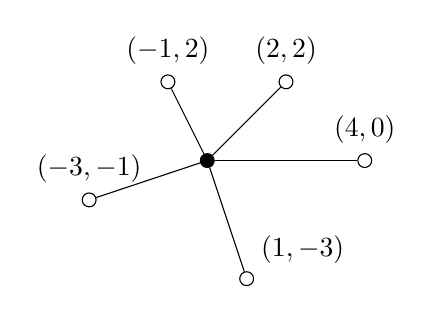
\begin{tikzpicture}
    \tikzstyle{node}=[circle,draw, minimum width=5pt, inner sep=0pt]
    \tikzstyle{root}=[fill=black]

    \node[node, root] (root) at (0,0) {};
    \node[node, label={$(-1, 2)$}] (a) at (-0.5, 1) {};
    \node[node, label={$(4, 0)$}] (b) at (2, 0) {};
    \node[node, label={$(2, 2)$}] (c) at (1, 1) {};
    \node[node, label={$(-3, -1)$}] (d) at (-1.5, -0.5) {};
    \node[node, label={50:$(1, -3)$}] (e) at (0.5, -1.5) {};

    \path (root) edge (a);
    \path (root) edge (b);
    \path (root) edge (c);
    \path (root) edge (d);
    \path (root) edge (e);
  \end{tikzpicture}
  \subcaption{Ursprüngliche Kantenattribute eines Knoten}
\end{subfigure}
\end{minipage}
\begin{minipage}[c]{0.49\textwidth}
\begin{subfigure}[c]{0.49\textwidth}
  \centering
  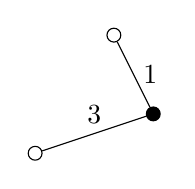
\begin{tikzpicture}
    \tikzstyle{node}=[circle,draw, minimum width=5pt, inner sep=0pt]
    \tikzstyle{root}=[fill=black]

    \node[node, root] (root) at (0,0) {};
    \node[node] (a) at (-0.5, 1) {};
    \node[node] (d) at (-1.5, -0.5) {};

    \path (root) edge[right] node {1} (a);
    \path (root) edge[above] node {3} (d);
  \end{tikzpicture}
  \subcaption{$A_{\text{links}}$}
\end{subfigure}
\begin{subfigure}[c]{0.49\textwidth}
  \centering
  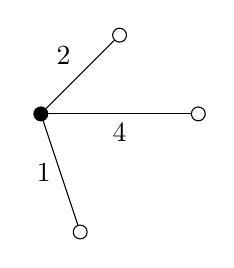
\begin{tikzpicture}
    \tikzstyle{node}=[circle,draw, minimum width=5pt, inner sep=0pt]
    \tikzstyle{root}=[fill=black]

    \node[node, root] (root) at (0,0) {};
    \node[node] (b) at (2, 0) {};
    \node[node] (c) at (1, 1) {};
    \node[node] (e) at (0.5, -1.5) {};

    \path (root) edge[below] node {4} (b);
    \path (root) edge[above left] node {2} (c);
    \path (root) edge[left] node {1} (e);
  \end{tikzpicture}
  \subcaption{$A_{\text{rechts}}$}
\end{subfigure}
\begin{subfigure}[c]{0.49\textwidth}
  \centering
  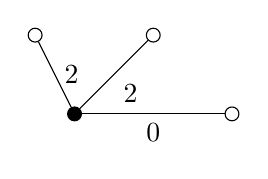
\begin{tikzpicture}
    \tikzstyle{node}=[circle,draw, minimum width=5pt, inner sep=0pt]
    \tikzstyle{root}=[fill=black]

    \node[node, root] (root) at (0,0) {};
    \node[node] (a) at (-0.5, 1) {};
    \node[node] (b) at (2, 0) {};
    \node[node] (c) at (1, 1) {};

    \path (root) edge[right] node {2} (a);
    \path (root) edge[below] node {0} (b);
    \path (root) edge[below right] node {2} (c);
  \end{tikzpicture}
  \subcaption{$A_{\text{oben}}$}
\end{subfigure}
\begin{subfigure}[c]{0.49\textwidth}
  \centering
  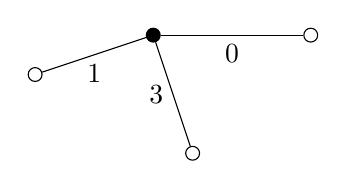
\begin{tikzpicture}
    \tikzstyle{node}=[circle,draw, minimum width=5pt, inner sep=0pt]
    \tikzstyle{root}=[fill=black]

    \node[node, root] (root) at (0,0) {};
    \node[node] (b) at (2, 0) {};
    \node[node] (d) at (-1.5, -0.5) {};
    \node[node] (e) at (0.5, -1.5) {};

    \path (root) edge[below] node {0} (b);
    \path (root) edge[below] node {1} (d);
    \path (root) edge[left] node {3} (e);
  \end{tikzpicture}
  \subcaption{$A_{\text{unten}}$}
\end{subfigure}
\end{minipage}
\caption{Aufteilung einer Adjazenzmatrix in vier räumliche Bereiche.}
\label{adjazenz_aufteilung}
\end{figure}

Kantenattribute bzw.\ Positionen von Knoten sollten skalierungsinvariant gespeichert werden.
Dafür werden die Abstände auf den Einheitskreis gemappt, wobei die längste Distanz eines Knotens auf dem Einheitskreis liegt (vgl. Abbildung~\ref{einheitskreis}).

\begin{figure}
\begin{tikzpicture}
  \draw[dashed] (0, 0) circle (4);

  \tikzstyle{node}=[circle,draw, minimum width=5pt, inner sep=0pt, fill=white]
  \tikzstyle{root}=[fill=black]

  \node[node, root] (root) at (0,0) {};
  \node[node, label={[fill=white]150:$(-1, 2) \rightarrow (-.25,.5)$}] (a) at (-1, 2) {};
  \node[node, label={[fill=white]$(4, 0) \rightarrow (1, 0)$}] (b) at (4, 0) {};
  \node[node, label={[fill=white]$(2, 2) \rightarrow (.5,.5)$}] (c) at (2, 2) {};
  \node[node, label={[fill=white]150:$(-3, -1) \rightarrow (-.75, -.25)$}] (d) at (-3, -1) {};
  \node[node, label={[fill=white]50:$(1, -3) \rightarrow (.25, -.75)$}] (e) at (1, -3) {};

  \path (root) edge (a);
  \path (root) edge (b);
  \path (root) edge (c);
  \path (root) edge (d);
  \path (root) edge (e);
\end{tikzpicture}
\caption{Abbildung der lokalen Nachbarschaftsknoten auf den Einheitskreis.}
\label{einheitskreis}
\end{figure}

Für die Anwendung auf das Graph Convolutional Network müssen die Gewichte aller Adjazenzmatrizen $a_{xij} \in [0, 1]$ invertiert werden, damit nähere Knoten einen größeren Einfluss haben.
Ebenso müssen \emph{Self Loops} für alle Knoten hinzugefügt werden.
Wir definieren unsere Adjazenzmatrix $\tilde A \in \mathbb{R}^{N \times N}$ aus einer Adjazenzmatrix $A \in \mathbb{R}^{N \times N}$ dann über

\begin{equation}
  \tilde A_{ij} = \begin{cases}
    1, & \text{falls }i=j\text{,}\\
    {(a_{ij}+1)}^{-1}, & \text{falls }a_{ij} \neq 0\text{,}\\
    0, & \text{sonst.}
  \end{cases}
\end{equation}

Dann ist $\tilde a_{ij} \in [1, 0.5]$

Diagonalmatrix ist schwierig.
Man will ja die Normalisierung damit $H^{(l)}$ nicht überskaliert.
Ich würde auch die gewichtete Matrix normalisieren.
Denke das macht Sinn.
Dann fallen die Werte ab, wenn viele Knoten weit entfernt sind.

\section{Erweiterung auf Graphen im zweidimensionalen Raum}
\label{gcn_erweiterung}

Die Ansätze von~\citeauthor{Defferrard} aus Kapitel~\ref{spektraler_faltungsoperator} und von~\citeauthor{gcn} aus Kapitel~\ref{graph_convolutional_networks} zeigen konkurrenzfähige Resultate auf einer Reihe von Datensätzen auf Graphen (\vgl{}~\cite{Defferrard, gcn}).
So erreicht das \gls{GCN} \zB{} in der teilweise-überwachten Knotenklassifizierung von \emph{Referenzgraphen}, \dhe{} einer Menge von Knoten, die Dokumente über eine Reihe von Bag-of-Words-Merkmalen repräsentieren und (ungerichtet) über dessen Referenzierungen miteinander verbunden sind, beachtliche Ergebnisse und schneidet in diesen sogar knapp besser ab als über die Tschebyschow-Approximation mit $K=2$ und $K=3$~\cite{gcn}.

Die spektrale Faltung auf Graphen entspricht einer Generalisierung der Faltung klassischer \glspl{CNN} auf zweidimensionalen Bildern~\cite{gcn_review}.
Es ist jedoch anzumerken, dass die spektrale Faltung im Gegensatz zur klassischen Faltung auf einem regulären Gitter insbesondere rotationsinvariant ist.
Das ist in der Regel für generelle Graphen keine Schwäche, schließlich kann den Knoten \bzw{} Kanten eines Graphen, kodiert als Adjazenzmatrix, keine Örtlichkeit \bzw{} Richtung (wie links, rechts, oben oder unten) zugeordnet werden.
Die Rotationsinvarianz kann folglich sowohl als Einschränkung als auch als Vorteil interpretiert werden, abhängig von dem Problem, welches man betrachtet~\cite{Defferrard}.

\begin{figure}[t]
\centering
\subfigure[Reguläres Gitter]{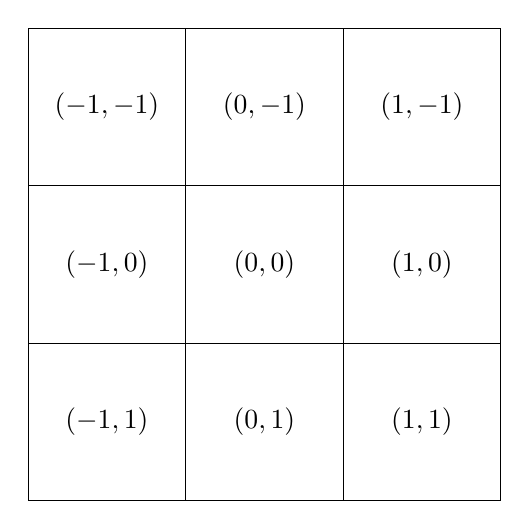
\begin{tikzpicture}
  \draw (-3, -3) rectangle (-1, -1) node[pos=0.5] {$\left(-1, 1\right)$};
  \draw (-1, -3) rectangle (1, -1)  node[pos=0.5] {$\left(0, 1\right)$};
  \draw (1, -3)  rectangle (3, -1)  node[pos=0.5] {$\left(1, 1\right)$};
  \draw (-3, -1) rectangle (-1, 1)  node[pos=0.5] {$\left(-1, 0\right)$};
  \draw (-1, -1) rectangle (1, 1)   node[pos=0.5] {$\left(0, 0\right)$};
  \draw (1, -1)  rectangle (3, 1)   node[pos=0.5] {$\left(1, 0\right)$};
  \draw (-3, 1)  rectangle (-1, 3)  node[pos=0.5] {$\left(-1, -1\right)$};
  \draw (-1, 1)  rectangle (1, 3)   node[pos=0.5] {$\left(0, -1\right)$};
  \draw (1, 1)   rectangle (3, 3)   node[pos=0.5] {$\left(1, -1\right)$};
\end{tikzpicture}
}
\hspace{1cm}
\subfigure[Graphrepräsentation]{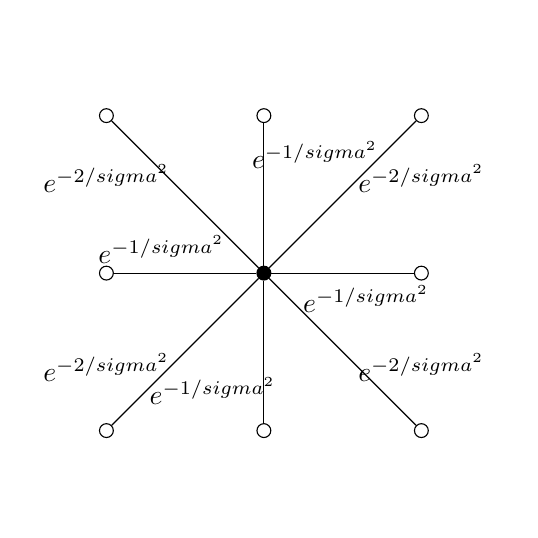
\begin{tikzpicture}
  \tikzstyle{node}=[circle,draw, minimum width=5pt, inner sep=0pt, fill=white]
  \tikzstyle{root}=[fill=black]
  \fill [white] (-3, -3) rectangle (3, 3) node {};  % Zentriere vertikal.

  \node[node] (00) at (-2, 2) {};
  \node[node] (01) at (0, 2) {};
  \node[node] (02) at (2, 2) {};
  \node[node] (10) at (-2, 0) {};
  \node[node, root] (11) at (0,0) {};
  \node[node] (12) at (2, 0) {};
  \node[node] (20) at (-2, -2) {};
  \node[node] (21) at (0, -2) {};
  \node[node] (22) at (2, -2) {};

  \path (10) edge node[shift={(-0.3, 0.3)}]  {$e^{-1/\gls{sigma}^2}$} (11);
  \path (11) edge node[shift={(0.3, -0.33)}]  {$e^{-1/\gls{sigma}^2}$} (12);
  \path (01) edge node[shift={(0.65, 0.5)}]   {$e^{-1/\gls{sigma}^2}$} (11);
  \path (11) edge node[shift={(-0.65, -0.5)}] {$e^{-1/\gls{sigma}^2}$} (21);
  \path (00) edge node[shift={(-1, 0.2)}]    {$e^{-2/\gls{sigma}^2}$} (11);
  \path (02) edge node[shift={(1, 0.2)}]     {$e^{-2/\gls{sigma}^2}$} (11);
  \path (11) edge node[shift={(1, -0.2)}]    {$e^{-2/\gls{sigma}^2}$} (22);
  \path (20) edge node[shift={(-1, -0.2)}]   {$e^{-2/\gls{sigma}^2}$} (11);
\end{tikzpicture}
}
  \caption[Graphrepräsentation eines regulären Gitters]{Illustration (a) eines $3 \times 3$ großen regulären Gitters zentriert um den Punkt $\left(0, 0\right)$ und (b) dessen lokale Nachbarschaft der entsprechenden Graphrepräsentation mit einer Konnektivität von $8$ bei horizontalen \bzw{} vertikalen Kantengewichten $\exp\left(-1/\gls{sigma}^2\right) \in \gls{R}$ \bzw{} $\exp\left(-2/\gls{sigma}^2\right) \in \gls{R}$ bei den Diagonalen.}
\label{fig:gcn_review}
\end{figure}


Im Kontext dieser Arbeit, dem Lernen auf Graphen im zweidimensionalen euklidischen Raum, bei denen Graphknoten eine eindeutige Position besitzen, ist die Rotationsinvarianz weitestgehend unerwünscht.
Das kann leicht verifiziert werden, indem wir den Filter des \glspl{GCN} auf einer Graphrepräsentation eines Gitters mit Abstand $\left\|1\right\|_2$ visualisieren (vgl. Abbildung~\ref{fig:gcn_review}).
Diese Repräsentation entspricht damit genau dem Problem der zweidimensionalen Faltung auf Bildern mit einer Filtergröße von $3 \times 3$.
Hier zeigt sich jedoch besonders deutlich die Limitierung des Netzes durch die Rotationsinvarianz.
Wohingegen wir bei klassischen \glspl{CNN} $3 \times 3$ unterschiedliche Parameter mit eindeutiger Örtlichkeit auf den benachbarten Bildpixeln trainieren, reduziert sich der Filter des \glspl{GCN} (vereinfacht ohne Normalisierung mit $\gls{Dtilde}^{-1/2}$) effektiv zu einer Filtermatrix der Form
\begin{equation*}
  \begin{bmatrix}
    ce^{-1/\gls{sigma}^2} & ce^{-0.5/\gls{sigma}^2} & ce^{-1/\gls{sigma}^2}\\
    ce^{-0.5/\gls{sigma}^2} & c & ce^{-0.5/\gls{sigma}^2}\\
    ce^{-1/\gls{sigma}^2} & ce^{-0.5/\gls{sigma}^2} & ce^{-1/\gls{sigma}^2}
  \end{bmatrix} = c \begin{bmatrix}
    e^{-1/\gls{sigma}^2} & e^{-0.5/\gls{sigma}^2} & e^{-1/\gls{sigma}^2}\\
    e^{-0.5/\gls{sigma}^2} & 1 & e^{-0.5/\gls{sigma}^2}\\
    e^{-1/\gls{sigma}^2} & e^{-0.5/\gls{sigma}^2} & e^{-1/\gls{sigma}^2}
  \end{bmatrix}
\end{equation*}
mit einem einzigen trainierbaren Parameter $c \in \gls{R}$ bei horizontalen \bzw{} vertikalen Kantengewichten nach~\eqref{gauss} mit $\exp\left(-0.5/\gls{sigma}^2\right) \in \gls{R}$ \bzw{} mit $\exp\left(-1/\gls{sigma}^2\right) \in \gls{R}$ bei den Diagonalen.
Damit reduziert sich das Training einer Faltungsschicht eines solchen \glspl{GCN} letztendlich auf eine Skalarmultiplikation.
Es scheint schwer vorstellbar mit diesem Ansatz komplexe Probleme wie \zB{} das Segmentieren eines Bildes zu lösen~(\vgl{}~\cite{gcn_review}).
Ein Vergleich zwischen der spektralen Faltung auf regulären Gittergraphen und der klassischen zweidimensionalen Faltung auf Bildern wird der spektralen Faltung aber nicht gerecht, schließlich wurden die klassischen \glspl{CNN} speziell für die Anwendung auf Gittern entwickelt.
So ist es zu erwarten, dass durch die Formulierung einer Faltung für generelle Graphen gewisse Einschränkungen in Kauf genommen werden müssen.
Im Folgenden lässt sich der Faltungsoperator der \glspl{GCN} aber insofern modifizieren, dass sich dieser für beliebige Graphen in einem zweidimensionalen euklidischen Raum äquivalent zu der klassischen Formulierung auf regulären Gittern verhält.

\subsection{Partitionierung}
\label{partitionierung}

\begin{figure}[t]
\centering
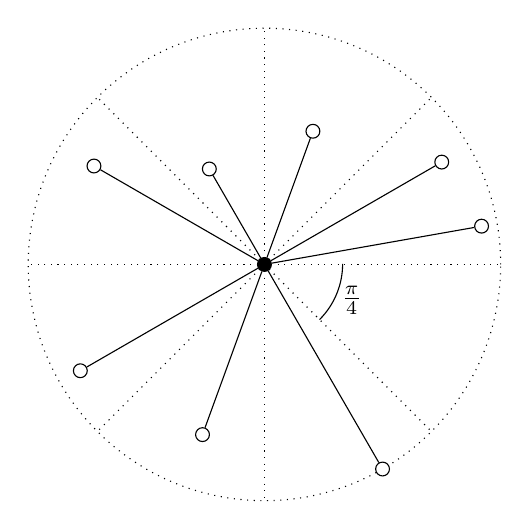
\begin{tikzpicture}
  % Kreis.
  \draw[dotted] (0, 0) circle (3);

  % Partitionierungen.
  \draw[dotted] (0, 0) -- (0:3);
  \draw[dotted] (0, 0) -- (45:3);
  \draw[dotted] (0, 0) -- (90:3);
  \draw[dotted] (0, 0) -- (135:3);
  \draw[dotted] (0, 0) -- (180:3);
  \draw[dotted] (0, 0) -- (225:3);
  \draw[dotted] (0, 0) -- (270:3);
  \draw[dotted] (0, 0) -- (315:3);

  % Graph.
  \tikzstyle{node}=[circle,draw, minimum width=5pt, inner sep=0pt, fill=white]
  \tikzstyle{root}=[fill=black]

  \node[node, root] (root) at (0,0) {};
  \node[node] (a) at (10:2.8) {};
  \node[node] (b) at (30:2.6) {};
  \node[node] (c) at (70:1.8) {};
  \node[node] (d) at (120:1.4) {};
  \node[node] (e) at (150:2.5) {};
  \node[node] (f) at (210:2.7) {};
  \node[node] (g) at (250:2.3) {};
  \node[node] (h) at (300:3) {};

  \path (root) edge (a);
  \path (root) edge (b);
  \path (root) edge (c);
  \path (root) edge (d);
  \path (root) edge (e);
  \path (root) edge (f);
  \path (root) edge (g);
  \path (root) edge (h);

  % Winkel.
  \coordinate (O) at (0, 0);
  \coordinate (A) at (2, 0);
  \coordinate (B) at (2, 2);

  \draw (0.7, -0.7) arc (-45:0:1);
  \node[] at (-22.5:1.2) {$\frac{\pi}{4}$};
\end{tikzpicture}
\caption[Partitionierung eines Graphknotens]{Partitionierung eines Graphknotens in $P = 8$ gleichmäßige Bereiche mit Innenwinkeln $\pi/4$.}
\label{fig:partitionierung}
\end{figure}


Sei \gls{G} ein Graph im zweidimensionalen euklidischen Raum, definiert über dessen Adjazenzmatrizen $\gls{Adist} \in {\left[0, 1\right)}^{N \times N}$ und $\gls{Arad} \in {\left[0, 2\pi\right]}^{N \times N}$ (\vgl{} Kapitel~\ref{graphrepraesentationen_von_bildern}).
Dann lässt sich \gls{G} in $P \in \gls{N}$ Bereiche ${\left\{\gls{A}_p\right\}}_{p=0}^{P-1}$ \emph{partitionieren}, sodass
\begin{equation*}
  {\left(\gls{A}_p\right)}_{ij} \coloneqq \begin{cases}
    {\left(\gls{Adist}\right)}_{ij}, & \text{wenn } {\left(\gls{Arad}\right)}_{ij} \in \left(2\pi p/P, 2\pi\left(p+1\right)/P\right],\\
    0, & \text{sonst.}
  \end{cases}
\end{equation*}
Damit beschreiben die Matrizen ${\left\{\gls{A}_p\right\}}_{p=0}^{P-1}$ disjunkte Partitionen der Kanten des Graphen \gls{G} abhängig von ihren Ausrichtungen im Raum mit $\gls{Adist} = \sum_{p=0}^{P-1} \gls{A}_p$.
$\gls{A}_p$ ist insbesondere nicht symmetrisch, da ${\left(\gls{Arad}\right)}_{ij} \neq {\left(\gls{Arad}\right)}_{ji}$ für alle $\gls{v}_i, \gls{v}_j \in \gls{V}$ mit $\gls{v}_j \in \gls{Neighbor}\left(\gls{v}_i\right)$.
Abbildung~\ref{fig:partitionierung} veranschaulicht den Prozess der Partitionierung.
Mit $P = 8$ erhalten die jeweiligen Bereiche \zB{} einen gleichmäßigen Innenwinkel der Größe $\pi/4$.

\paragraph{Faltungsoperator}
\label{partitionierung_faltungsoperator}

Es lässt sich analog zu Kapitel~\ref{graph_convolutional_networks} ein Faltungsoperator definieren, bei dem nun jeder Partition ein eigener frei trainierbarer Parameter zugeordnet wird.
Der Parameter einer Partition hat damit folglich eine eindeutige Örtlichkeitszuweisung über das Intervall \bzw{} den Bereich der Richtungen seiner Kanten.
Analog zu~\eqref{eq:gcn_renorm} muss dafür zuerst die (Re-)normalisierung der Form
\begin{equation*}
  \gls{Ddisttilde}^{-\frac{1}{2}}\gls{Adisttilde}\gls{Ddisttilde}^{-\frac{1}{2}} = \gls{Ddisttilde}^{-1} + \sum_{p=0}^{P-1} \gls{Ddisttilde}^{-\frac{1}{2}}\gls{A}_p\gls{Ddisttilde}^{-\frac{1}{2}}
\end{equation*}
mit $\gls{Adisttilde} \coloneqq \gls{Adist} + \gls{I}$ und ${\left(\gls{Ddisttilde}\right)}_{ii} \coloneqq \sum_{j=1}^N {\left(\gls{Adisttilde}\right)}_{ij}$ durchgeführt werden.
Dies lässt sich mit Hilfe von $\gls{Adist} = \sum_{p=0}^{P-1} \gls{A}_p$ und $\gls{Ddisttilde}^{-1/2}\gls{Ddisttilde}^{-1/2} = \gls{Ddisttilde}^{-1}$ verifizieren.
Im Folgenden sei $\gls{Atilde}_p \coloneqq \gls{Ddisttilde}^{-1/2}\gls{A}_p\gls{Ddisttilde}^{-1/2}$ für $p \in \left\{0, \ldots, P-1 \right\}$ und $\gls{Atilde}_P \coloneqq \gls{Ddisttilde}^{-1}$.
Dann folgt für den Faltungsoperatur $\gls{f}_{\mathrm{in}} \star \ve{\hat g}$ auf Graphen im zweidimensionalen euklidischen Raum, dass dieser über
\begin{equation}
  \gls{f}_{\mathrm{in}} \star \ve{\hat g} \approx \sum_{p=0}^P c_p \gls{Atilde}_p \gls{f}_{\mathrm{in}}
  \label{eq:partitionierung_faltung}
\end{equation}
mit den freien Parametern ${\left[c_0, \ldots, c_P\right]}^{\top} \in \gls{R}^{P+1}$ beschrieben werden kann.
\\\\
Es stellt sich heraus, dass die Faltung in~\eqref{eq:partitionierung_faltung} auf den Partitionen eines regulären Gittergraphen mit $P=8$ äquivalent zu der klassischen Faltung auf einem regulären Gitter mit Filtergröße $3 \times 3$ ist.
Sei dafür \gls{G} ein (unendlicher) regulärer Gittergraph bei einer Konnektivität von $8$ und $\gls{f}_{\mathrm{in}}$ Merkmalsvektor auf dem Graphen mit Koordinatenindexnotation ${\left(\gls{f}_{\mathrm{in}}\right)}_{x,y}$.
  Die klassische Faltung \gls{conv2d} an einem Gitterpunkt $\left(x, y\right)$ ist damit gegeben als
\begin{equation*}
  {\gls{conv2d}\left({\gls{f}_{\mathrm{in}}}\right)}_{x,y} = \sum_{i,j \in \left\{1, 2, 3\right\}} {\left(\gls{f}_{\mathrm{in}}\right)}_{x+i-2, y+j-2} \gls{W}_{i, j},
\end{equation*}
wobei $\gls{W} \in \gls{R}^{3 \times 3}$ eine Filtermatrix der Größe $3 \times 3$ ist.
Da \gls{Adisttilde} ein reguläres Gitter beschreibt sind die Einträge ihrer Matrixreihen äquivalent unter unterschiedlicher Permutation und folglich sind die Einträge auf der Diagonalen von \gls{Ddisttilde} identisch (\oBdA{} entfällt hier die Randknotenbetrachtung).
Aufgrund der Partitionierung von \gls{Adist} in $8$ disjunkte Bereiche ${\left\{\gls{Atilde}_p\right\}}_{p=0}^7$ enthält $\gls{Atilde}_p$ genau einen Eintrag pro Matrixreihe korrespondierend zu einer Kante des regulären Gitters.
Für $p \in \left\{1, 3, 5, 7\right\}$ beschreibt $\gls{Atilde}_p$ die horizontalen und vertikalen Kanten des Graphen mit jeweils gleichen Einträgen $\theta_0 \in \gls{R}$.
Analog verweist $\gls{Atilde}_p$ für $p \in \left\{0, 2, 4, 6\right\}$ auf die diagonalen Kanten des Graphen mit den festen Einträgen $\theta_1 \in \gls{R}$.
Sei weiterhin \oBdA{} $\theta_2 \coloneqq {\left(\gls{Ddisttilde}^{-1}\right)}_{ii}$ für beliebiges $i \in \left\{0, \ldots, N\right\}$.
Mit der Zuordnung
\begin{equation*}
  \gls{W} = \begin{bmatrix}
    c_6\theta_1 & c_7\theta_0 & c_0\theta_1\\
    c_5\theta_0 & c_8\theta_2 & c_1\theta_0\\
    c_4\theta_1 & c_3\theta_0 & c_2\theta_1
  \end{bmatrix}
\end{equation*}
  für den Faltungsoperator $\gls{f}_{\mathrm{in}} \star \ve{\hat g}$ aus~\eqref{eq:partitionierung_faltung} mit den Parametern ${\left[c_0, \ldots, c_8\right]}^{\top} \in \gls{R}^9$
folgt damit sofort die Äquivalenz zu $\gls{conv2d}\left(\gls{f}_{\mathrm{in}}\right)$ auf regulären Gittern.

\paragraph{Implementierung}
\label{partitionierung_implementierung}

Analog zu~\eqref{eq:gcn_tensor} lässt sich die Faltung für Merkmalsmatrizen $\gls{F}_{\mathrm{in}} \in \gls{R}^{N \times M_{\mathrm{in}}}$ und $\gls{F}_{\mathrm{out}} \in \gls{R}^{N \times M_{\mathrm{out}}}$ über einem Filtertensor $\gls{W} \in \gls{R}^{\left(P+1\right) \times M_{\mathrm{in}} \times M_{\mathrm{out}}}$ als
\begin{equation*}
  \gls{F}_{\mathrm{out}} \coloneqq \sum_{p=0}^P \gls{Atilde}_p\gls{F}_{\mathrm{in}}\gls{W}_{p+1}
\end{equation*}
beschreiben.
Es ist anzumerken, dass die Multiplikation mit den dünnbesetzten partitionierten Adjazenzmatrizen ${\left\{\gls{Atilde}_p\right\}}_{p=0}^P$ extrem effizient ist, da $\left|\gls{E}_p\right| \ll \left|\gls{E}\right|$ und insbesondere $\sum_{p=0}^P \left|\gls{E}_p\right| = \left|\gls{E}\right| + N$ gilt, wobei $\gls{E}_p \in \gls{V} \times \gls{V}$ die Kantenmenge der Adjazenzmatrix $\gls{Atilde}_p$ beschreibt.
Die Laufzeit erhöht sich jedoch im Vergleich zu~\eqref{eq:gcn_tensor} durch die $P$-fache Multiplikation mit der Filtermatrix $\gls{W}_p$ zu $\gls{O}\left(PM_{\mathrm{in}}M_{\mathrm{out}}\left|\gls{E}\right|\right)$.
\\\\
Obwohl die Faltung auf den Partitionen eines Graphen insbesondere durch die Äquivalenz zur klassischen Faltung auf regulären Gittern vielversprechend erscheint, gehen dabei dennoch Informationen über die Ausrichtung der Kanten im Raum verloren.
Kanten mit verschiedenen Richtungen im Intervall $\left(2\pi p/P, 2\pi \left(p+1\right)/P\right]$ landen jeweils in der gleichen Partition $p$, auch wenn sich diese \evtl{} extrem unterscheiden.
Eine Lösung zu diesem Problem ist sicherlich, $P$ insoweit zu erhöhen, dass die Innenwinkel der einzelnen Partitionen entsprechend klein werden.
Dies erscheint jedoch für beliebige, unbekannte Graphstrukturen nicht zwangsläufig sinnvoll.
Neben dem erhöhten Aufwand der Faltung erhalten wir im schlimmsten Fall viele Partitionsmatrizen $\gls{A}_p$, die eine Nullmatrix \ma{0} darstellen oder nur extrem wenige Kanten beinhalten.
Kleinste Veränderungen in den Ausrichtungen der Kanten sorgen dann schließlich dafür, dass eine komplett andere Filtermatrix angesprochen wird.
Ein dazu alternativ entwickelter Ansatz ist die Approximation des Filters über stückweise stetiger Polynome zwischen den Partitionsgrenzen des Graphen mit Hilfe von B-Spline-Kurven.

\subsection{Polynomielle Approximation über B-Spline-Kurven}
\label{bspline}

Eine B-Spline-Kurve beschreibt eine stückweise polynomielle Approximation einer Kurve vom Grad $K \in \gls{N}$ über $M + 1$ Kontrollpunkten $\ve{d}_0, \ldots, \ve{d}_M \in \gls{R}^d$~\cite{deBoor}.
Eine B-Spline Kurve kann dabei offen, \dhe{} mit beliebigen Endpunkten, sowie geschlossen, \dhe{} mit gleichem Anfangs- und Endpunkt, beschrieben werden~\cite{gm}.
Die \emph{geschlossene B-Spline-Kurve} $\gls{spline}\left(t\right)$ ist auf dem Intervall $t \in \left(t_0, t_{M+1}\right]$ definiert als
\begin{equation}
  \gls{spline}\left(t\right) \coloneqq \sum_{m = 0}^M \ve{d}_m \gls{basis}_m^K\left(t\right),
    \label{eq:bspline}
\end{equation}
mit den \emph{B-Spline-Funktionen} ${\left\{\gls{basis}_m^K\right\}}_{m=0}^M$ zu einem \emph{Knotenvektor} $\ve{\tau} \in \gls{R}^{M+K+2}$ der Form $\ve{\tau} \coloneqq {\left[t_0, \ldots, t_{M+K+1}\right]}^{\top}$ mit der Bedingung, dass $t_{M+k+2} \coloneqq t_{M+k+1} + \left(t_{k+1} - t_k\right)$ für $k \in \left\{0, \ldots, K-1\right\}$~\cite{gm}.
Die B-Spline-Funktion $\gls{basis}_m^K \colon \left(t_0, t_{m+1}\right] \to \left[0, 1\right]$ ist rekursiv über $k \in \left\{0, \ldots, K \right\}$ definiert mit der Initialisierung ($k=0$)
\begin{equation*}
  \gls{basis}_m^0\left(t\right) \coloneqq \begin{cases}
    1, & \text{falls }t \in \left(t_m, t_{m+1}\right],\\
    0, & \text{sonst}
  \end{cases}
\end{equation*}
und dem Rekursionsschritt ($k - 1 \rightarrow k$)
\begin{equation*}
  \gls{basis}_m^k\left(t\right) \coloneqq \frac{t-t_m}{t_{m+k} - t_m}\gls{basis}^{k-1}_m\left(t\right) + \frac{t_{m+k+1} - t}{t_{m+k+1} - t_{m+1}} \gls{basis}_{m+1}^{k-1}\left(t\right)
\end{equation*}
für $t \in \left(t_m, t_{M+1}\right]$ sowie $\gls{basis}_m^k\left(t\right) \coloneqq \gls{basis}_m^k\left(t - t_0 + t_{M+1}\right)$ für $t \in \left(t_0, t_m\right]$~\cite{gm}.
Ein Kontrollpunkt $\ve{d}_m$ beeinflusst die Kurve damit lediglich im Intervall $t_m < t \leq t_{m+K+1}$.
Die Größe von $K$ wird deshalb auch oft \emph{lokale Kontrollierbarkeit} genannt.
Weiterhin gilt für die Aufsummierung der B-Spline-Funktionen ${\left\{\gls{basis}_m^K\right\}}_{m=0}^M$, dass $\sum_{m=0}^M \gls{basis}_m^K\left(t\right) = 1$ für beliebige $K \in \gls{N}$ und $t \in \left(t_0, t_{M+1}\right]$~\cite{deBoor}.

Wir können die Definition der B-Spline-Kurve $\gls{spline}\left(t\right)$ aus~\eqref{eq:bspline} nutzen, um sie aufbauend auf Kapitel~\ref{partitionierung} in das Anwendungsgebiet eines stückweisen polynomiellen Filters $\gls{spline}\left(\alpha\right)$ auf den Richtungen \bzw{} Winkeln eines Graphen \gls{G}, beschrieben durch \gls{Adist} und \gls{Arad}, zu übertragen.
Sei dafür $\gls{spline} \colon \left[0, 2\pi\right] \to \gls{R}$ im Folgenden eine B-Spline-Kurve auf den Winkeln der Graphkanten mit
\begin{equation*}
  \gls{spline}\left(\alpha\right) \coloneqq \sum_{p=0}^{P-1} c_p N_p^K\left(\alpha\right),
\end{equation*}
wobei die freien Parameter ${\left[c_0, \ldots, c_{P-1}\right]}^{\top} \in \gls{R}^{P}$ aus~\eqref{eq:partitionierung_faltung} nun die Koeffizienten der B-Spline-Funktionen ${\left\{N_p^K\right\}}_{p=0}^{P-1}$ bilden.
Insbesondere definieren wir $\gls{spline}\left(0\right) \coloneqq 0$, da der Winkel $0$ in der Adjazenzmatrix $\gls{Arad}$ weiterhin angeben soll, dass $\left(\gls{v}_i, \gls{v}_j\right) \notin \gls{E}$.
Wir können uns $\gls{spline}\left(\alpha\right)$ damit weiterhin als eine $P$-fache Partitionierung von \gls{G} auf Basis seiner Kantenausrichtungen vorstellen, mit dem Unterschied, dass $\gls{spline}\left(\alpha\right)$ nun eine lokale Kontrollierbarkeit inne hält.
Kanten, die vorher zwar in einer gleichen Partition lagen, sich jedoch \evtl{} stark in ihrer Ausrichtung unterschieden, sind nun \enquote{eindeutig} differenzierbar über ihre abweichenden Auswertungen von ${\left\{\gls{basis}_p^K\right\}}_{p=0}^{P-1}$ \bzw{} ihrer Anteile von ${\left[c_0, \ldots, c_{P-1}\right]}^{\top}$ an $\gls{spline}\left(\alpha\right)$ entsprechend ihrer unterschiedlichen Winkel.
Abbildung~\ref{fig:bspline} soll dabei das Konzept geschlossener B-Spline-Funktionen auf Winkeln veranschaulichen.
\begin{figure}[t]
\centering
\subfigure[$K=1$]{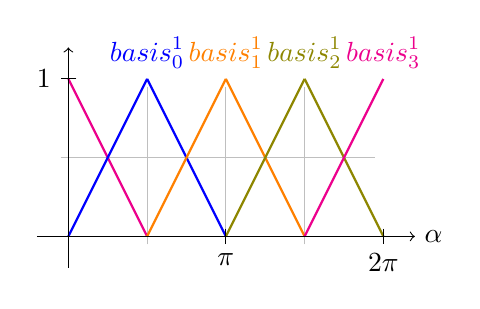
\begin{tikzpicture}
  \draw[color=lightgray] (-0.1, -0.1) grid (3.9, 1.9);

  \draw[thick,color=magenta] (0, 2) -- (1, 0);
  \draw[thick,color=blue] (0, 0) -- (1, 2) node[above] {$\gls{basis}_0^1$};
  \draw[thick,color=blue] (1, 2) -- (2, 0);
  \draw[thick,color=orange] (1, 0) -- (2, 2) node[above] {$\gls{basis}_1^1$};
  \draw[thick,color=orange] (2, 2) -- (3, 0);
  \draw[thick,color=olive] (2, 0) -- (3, 2) node[above] {$\gls{basis}_2^1$};
  \draw[thick,color=olive] (3, 2) -- (4, 0);
  \draw[thick,color=magenta] (3, 0) -- (4, 2) node[above] {$\gls{basis}_3^1$};

  \draw[->] (-0.4, 0) -- (4.4, 0) node[right] {$\alpha$};
  \draw[->] (0, -0.4) -- (0, 2.4);
  \draw (0.1, 2) -- (-0.1, 2) node[left] {$1$};
  \draw (2, 0.1) -- (2, -0.1) node[below] {$\pi$};
  \draw (4, 0.1) -- (4, -0.1) node[below] {$2\pi$};

  \end{tikzpicture}
}
\hspace{1cm}
\subfigure[$K=2$]{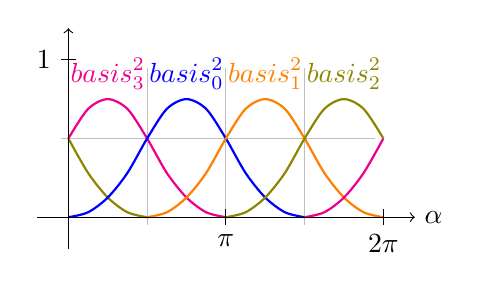
\begin{tikzpicture}
  \draw[color=lightgray] (-0.1, -0.1) grid (3.9, 1.9);

  \draw[color=blue] (1.5,1.5) node[above] {$\gls{basis}_0^2$};
  \draw[color=orange] (2.5,1.5) node[above] {$\gls{basis}_1^2$};
  \draw[color=olive] (3.5,1.5) node[above] {$\gls{basis}_2^2$};
  \draw[color=magenta] (0.5,1.5) node[above] {$\gls{basis}_3^2$};
  \draw[thick,color=magenta] plot [smooth] coordinates {(0,1)(0.25,1.375)(0.5,1.5)(0.75,1.375)(1,1)(1.25,0.5625)(1.5,0.25)(1.75,0.0625)(2,0)};
  \draw[thick,color=olive] plot [smooth] coordinates {(0,1)(0.25,0.5625)(0.5,0.25)(0.75,0.0625)(1,0)};
  \draw[thick,color=blue] plot [smooth] coordinates {(0,0)(0.25,0.0625)(0.5,0.25)(0.75,0.5625)(1,1)(1.25,1.375)(1.5,1.5)(1.75,1.375)(2,1)(2.25,0.5625)(2.5,0.25)(2.75,0.0625)(3,0)};
  \draw[thick,color=orange] plot [smooth] coordinates {(1,0)(1.25,0.0625)(1.5,0.25)(1.75,0.5625)(2,1)(2.25,1.375)(2.5,1.5)(2.75,1.375)(3,1)(3.25,0.5625)(3.5,0.25)(3.75,0.0625)(4,0)};
  \draw[thick,color=olive] plot [smooth] coordinates {(2,0)(2.25,0.0625)(2.5,0.25)(2.75,0.5625)(3,1)(3.25,1.375)(3.5,1.5)(3.75,1.375)(4,1)};
  \draw[thick,color=magenta] plot [smooth] coordinates {(3,0)(3.25,0.0625)(3.5,0.25)(3.75,0.5625)(4,1)};

  \draw[->] (-0.4, 0) -- (4.4, 0) node[right] {$\alpha$};
  \draw[->] (0, -0.4) -- (0, 2.4);
  \draw (0.1, 2) -- (-0.1, 2) node[left] {$1$};
  \draw (2, 0.1) -- (2, -0.1) node[below] {$\pi$};
  \draw (4, 0.1) -- (4, -0.1) node[below] {$2\pi$};

  \end{tikzpicture}
}
\caption[Geschlossene B-Spline-Basisfunktionen]{Illustration geschlossener Basisfunktionen $\gls{basis}_p^K \colon \left(0, 2\pi\right] \to \left[0, 1\right]$ für $P=4$ gleichmäßig verteilter Kontrollpunkte, einmal mit lokaler Kontrollierbarkeit $K=1$ (a) und einmal mit $K=2$ (b).}
\label{fig:bspline}
\end{figure}

Mit der expliziten Forderung gleichmäßig verteiler Knoten im Intervallbereich ergibt sich dann der Knotenvektor $\ve{\tau} \coloneqq {\left[\alpha_0, \ldots, \alpha_{P+K}\right]}^{\top} \in \gls{R+}^{P+K+1}$ mit $\alpha_p \coloneqq 2\pi p/P$ und erfüllt damit insbesondere die Bedingungen aus~\eqref{eq:bspline}.

\paragraph{Faltungsoperator}
\label{bspline_faltungsoperator}

Es kann folglich analog zu~\eqref{eq:partitionierung_faltung} der Faltungsoperator $\gls{f}_{\mathrm{in}} \star \ve{\hat g}$ auf Basis eines stückweisen polynomiellen Filters beschrieben werden.
Mit $\gls{Adisttilde} \in \gls{R}^{N \times N}$ und $\gls{Ddisttilde} \in \gls{R}^{N \times N}$ ergibt sich $\gls{f}_{\mathrm{in}} \star \ve{\hat g}$ dann als
\begin{equation*}
  \gls{f}_{\mathrm{in}} \star \ve{\hat g} \approx c_P \gls{Ddisttilde}^{-1}\gls{f}_{\mathrm{in}} + \sum_{p=0}^{P-1} \left(\left(c_p \gls{basis}_p^K\left(\gls{Arad}\right)\right)\gls{hadamard}\left(\gls{Ddisttilde}^{-\frac{1}{2}}\gls{Adisttilde}\gls{Ddisttilde}^{-\frac{1}{2}}\right)\right)\gls{f}_{\mathrm{in}}
\end{equation*}
mit den freien Parametern ${\left[c_0, \ldots, c_P\right]}^{\top} \in \gls{R}^{P+1}$, wobei $\gls{basis}_p^K$ elementweise auf die Matrix \gls{Arad} angewendet wird.
$\gls{f}_{\mathrm{in}} \star \ve{\hat g}$ sammelt dabei die aktuellen Merkmale an den einzelnen Knoten über $c_P \gls{Ddisttilde}^{-1}\gls{f}_{\mathrm{in}}$ und aggreriert diese mit den Merkmalen der lokalen Nachbarschaft über den polynomiellen Filter $\left(c_p\gls{basis}_p^K \left(\gls{Arad}\right)\right) \gls{hadamard} \left(\gls{Ddisttilde}^{-1/2}\gls{Adisttilde}\gls{Ddisttilde}^{-1/2}\right)$, der so die Länge und Richtungen der Kanten berücksichtigt.
Für $K=0$ ist die Faltung über den B-Splines äquivalent zu der Faltung über den Partitionen des Graphen aus~\eqref{eq:partitionierung_faltung} aufgrund der Rechteckfunktionen ${\left\{\gls{basis}_p^0\right\}}_{p=0}^{P-1}$.

\paragraph{Implementierung}
\label{bspline_implementierung}

Für Merkmalsmatrizen $\gls{F}_{\mathrm{in}} \in \gls{R}^{N \times M_{\mathrm{in}}}$ und $\gls{F}_{\mathrm{out}} \in \gls{R}^{N \times M_{\mathrm{out}}}$ kann die Faltung über einem Filtertensor $\gls{W} \in \gls{R}^{\left(P+1\right) \times M_{\mathrm{in}} \times M_{\mathrm{out}}}$ damit als
\begin{equation*}
  \gls{F}_{\mathrm{out}} \coloneqq \gls{Ddisttilde}^{-1}\gls{F}_{\mathrm{in}}\gls{W}_{P+1} + \sum_{p=0}^{P-1} \left(\gls{basis}_p^K\left(\gls{Arad}\right) \gls{hadamard}\left(\gls{Ddisttilde}^{-\frac{1}{2}}\gls{Adisttilde}\gls{Ddisttilde}^{-\frac{1}{2}}\right)\right)\gls{F}_{\mathrm{in}}\ma{W}_{p+1}
\end{equation*}
beschrieben werden.
Im Vergleich zu Kapitel~\eqref{partitionierung_implementierung} erhöht sich der Aufwand der Faltung zu $\gls{O}\left(KPM_{\mathrm{in}}M_{\mathrm{out}}\right)$, da die Partitionen der Adjazenzmatrizen nicht mehr disjunkt, sondern $\left(K+1\right)$-mal betrachtet werden.

\begin{figure}[t]
\centering
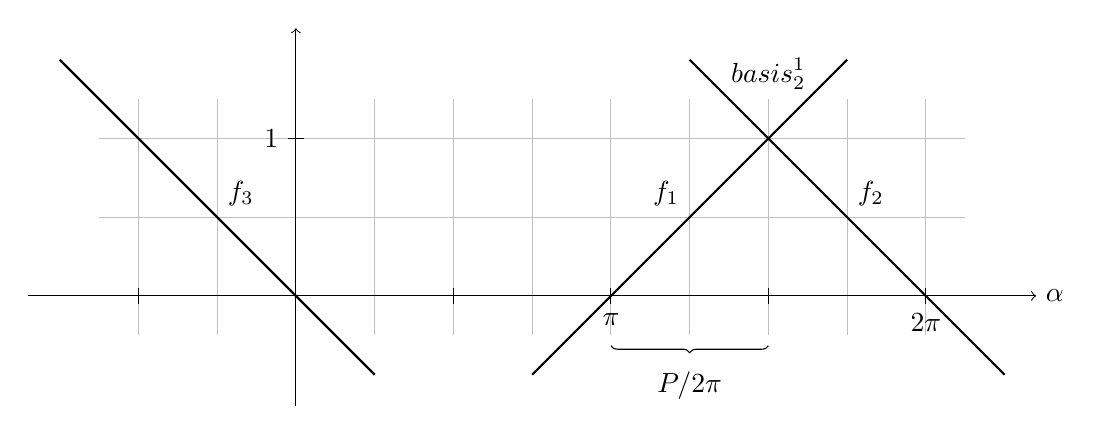
\begin{tikzpicture}
  \draw[color=lightgray] (-2.5, -0.5) grid (8.5, 2.5);

  \draw[thick] (3, -1) -- node[shift={(-0.3,0.3)}] {$f_1$} (7, 3);
  \draw[thick] (9, -1) -- node[shift={(0.3,0.3)}]  {$f_2$} (5, 3);
  \draw[thick] (1, -1) -- node[shift={(0.3,0.3)}]  {$f_3$} (-3, 3);

  \draw[->] (-3.4, 0) -- (9.4, 0) node[right] {$\alpha$};
  \draw[->] (0, -1.4) -- (0, 3.4);
  \draw (0.1, 2) -- (-0.1, 2) node[left] {$1$};
  \draw (-2, 0.1) -- (-2, -0.1);
  \draw (2, 0.1) -- (2, -0.1);
  \draw (4, 0.1) -- (4, -0.1) node[below] {$\pi$};
  \draw (6, 0.1) -- (6, -0.1);
  \draw (8, 0.1) -- (8, -0.1) node[below] {$2\pi$};

  \draw (6,2.5) node[above] {$\gls{basis}_2^1$};

  \draw [decoration={brace,mirror,raise=18pt},decorate] (4,0) -- node[below=24pt] {$P/2\pi$} (6,0);

\end{tikzpicture}
  \caption[B-Spline-Basisfunktion über Minimum-Maximumfunktionen]{Beweisidee zur kreisförmigen Dreiecksfunktion für B-Spline-Basis\-funk\-ti\-onen mit $K=1$ als Darstellung über eine Minimum-Maximumfunktion auf drei Geraden, hier illustriert am Beispiel $\gls{basis}_2^1$.}
\label{fig:bspline_beweis}
\end{figure}


Für $K=1$ lässt sich weiterhin die \enquote{kreisförmige} Dreiecksfunktion $\gls{basis}_p^1\left(\alpha\right)$ aus einer Reihe von Minimum- und Maximumfunktionen effizient implementieren.
So gilt, dass $\gls{basis}_p^1\left(\alpha\right)$ zu
\begin{equation*}
  \begin{split}
    \gls{basis}_p^1\left(\alpha\right) = \max \Big( & \min \left( \max\left(\frac{P}{2\pi}\alpha - p, 0\right), \max\left(-\frac{P}{2\pi}\alpha + p + 2, 0\right)\right),\\
    & \max\left(-\frac{P}{2\pi}\alpha + p + 2 - P, 0\right) \Big)
  \end{split}
\end{equation*}
vereinfacht werden kann.
Dies lässt sich verifizieren, in dem die kreisförmige Dreiecksfunktion im Intervall $\left(0, 2\pi\right]$ als Verknüpfung dreier Geraden verstanden wird — zwei Geraden, die das Dreieck im Intervall $\left(2\pi p/P, 2\pi \left(p+2\right)/P\right]$ aufspannen, und einer absteigenden Geraden, die um $2\pi$ nach links verschoben wurde und dafür sorgt, die B-Spline-Funktion für $p=P-1$ kreisförmig abzuschließen und in allen anderen Fällen keinen Anteil im Gültigkeitsbereich der Funktion $\gls{basis}_p^1 \colon \left(0,2\pi\right] \to \left[0,1\right]$ besitzt (\vgl{} Abbildung~\ref{fig:bspline_beweis}).
Den Geraden kann die Steigung $P/2\pi$ \bzw{} $-P/2\pi$ zugeordnet werden und sie können damit folglich über
\begin{equation*}
\begin{split}
  f_1\left(\alpha\right) \coloneqq & \frac{P}{2\pi}\left(\alpha - 2\pi\frac{p}{P}\right) = \frac{P}{2\pi}\alpha - p\\
  f_2\left(\alpha\right) \coloneqq & - \frac{P}{2\pi}\left(\alpha - 2\pi\frac{p+2}{P}\right) = - \frac{P}{2\pi}\alpha + p + 2\\
  f_3\left(\alpha\right) \coloneqq & - \frac{P}{2\pi}\left(\alpha - 2\pi\frac{p+2}{P} + 2\pi\right) = - \frac{P}{2\pi}\alpha + p + 2 - P
\end{split}
\end{equation*}
beschrieben werden.
Mittels $\max\left(f_i\left(\alpha\right), 0\right) \in \gls{R+}$ können diese auf den positiven reellen Raum eingegrenzt werden.
$f_{\triangle} \coloneqq \min\left(\max\left(f_1, 0\right), \max\left(f_2, 0\right)\right)$ beschreibt damit die Dreiecksfunktion, indem sie sich stets für das Minimum von $\max\left(f_1, 0\right)$ \bzw{} $\max\left(f_2,0\right)$ entscheidet.
Folglich beschreibt $\max\left(\max\left(f_3,0\right), f_{\triangle}\right)$ die B-Spline-Funktion $\gls{basis}_p^1$ im Intervall $\left(0, 2\pi\right]$ für alle $p \in \left\{0, \ldots, P-1\right\}$.

\section{Pooling auf Graphen}
\label{pooling}

\subsection{Graphvergröberung}
\label{graphvergroeberung}

\paragraph{Clustering von Knoten}
\label{clustering_von_knoten}

\subsection{Erweiterung auf ebene Graphen}
\label{pooling_erweiterung}

\section{Netzarchitektur}
\label{spektrale_netzarchitektur}

Die Architektur eines neuronalen Netzes auf Graphen mit spektralen Faltungen verhält sich durch die ähnliche Formulierung einer Faltungs- und einer Poo\-ling\-sch\-icht analog zu der Netzarchitektur klassischer \glspl{CNN}.
Dabei werden wie gewohnt mehrere Faltungsschichten mit stetig erhöhter Merkmalsausbreitung aneinander gereiht und an einigen Stellen über Poolingschichten getrennt, die die Anzahl der zu betrachtenden Knoten sukzessive reduzieren.
Im Anschluss darauf finden sich im Allgemeinen zwei bis drei vollverbundene Schichten, die die Merkmalsgröße dann schlussendlich auf die gewünschte Ausgabegröße reduzieren~\cite{Nielsen}.
Die mehrmalige Verkettung von Faltungsschichten sorgt dafür, dass auch bei einer relativ kleinen Faltung über die lokale Nachbarschaft eines jeden Knoten Merkmale weit entfernterer Knoten gewonnen werden können.

\glspl{CNN} auf Bildern erfordern dabei in einer analogen Netzarchitektur eine feste Eingabegröße.
Dafür werden die Bildermengen in der Regel insofern skaliert und zugeschnitten, dass diese alle die gleiche Bildgröße besitzen (\zB{} $224 \times 224$)~\cite{spp}.
Es erscheint jedoch schwierig, eine Menge von Graphen soweit anzupassen, dass diese alle die gleiche Anzahl an Knoten aufweisen.
So ist es zwar vorstellbar, zusätzliche \enquote{Fake}-Knoten zu jedem Graphen hinzufügen, damit diese alle eine feste Anzahl an Knoten aufweisen.
Neben dem erhöhtem Speicheraufwand ist dieser Ansatz jedoch insbesondere nicht geeignet für unbekannte Graphen, die in das Netz eingespeist werden.
So können diese \evtl{} eine größere Anzahl als die zuvor festgelegte Größe aufweisen.
Ebenso liefert uns der Prozess der Graphvergröberung eine stets unterschiedliche Repräsentation eines Graphen, die wohlmöglich bereits eine größere Menge an \enquote{Fake}-Knoten hinzufügt und dabei die festgelegte Knotengröße der Graphen überschreitet.
Es ist weiterhin schwierig, einen Graphen auf eine feste Größe zuzuschneiden.
So ist es insbesondere nicht ersichtlich, welche Knoten aus einem Graphen entfernt oder zusammengefasst werden können.

Die Architektur eines neuronalen Netzes auf Graphen erfordert folglich eine Struktur, die auf dynamischen Eingabegrößen operiert.
Dazu muss vorerst geklärt werden, warum ein klassisches \gls{CNN} auf Bildern eine feste Eingabegröße erfordert.
Eine einfache und elegante Lösung dazu bietet uns das \emph{Average-Pooling}, \dhe{} die Durchschnittsbildung eines Merkmals über allen Knoten.
Da die Anzahl der betrachteten Merkmale pro Knoten in jeder Schicht fest ist, liefert uns das Average-Pooling zwischen den Faltungs- und den vollverbundenen Schichten eines Netzes


Abbildung~\ref{fig:netzarchitektur_spectal} veranschaulicht die beschriebene typische spektrale Netzarchitektur.
\begin{figure}[t]
\centering
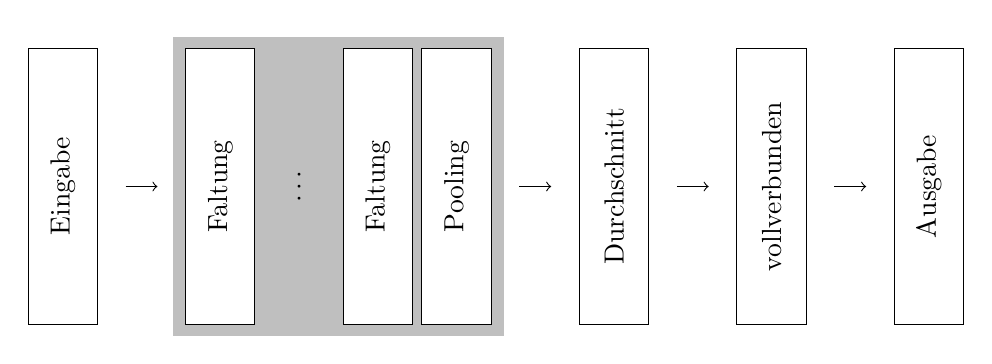
\begin{tikzpicture}[->, shorten >= 10pt, shorten <= 10pt]
  \tikzstyle{node}=[rectangle,draw, minimum width=100pt, minimum height=25pt, inner sep=0pt, fill=white, rotate=90]
  \tikzstyle{noborder}=[draw=none,fill=none]
  \tikzstyle{color1}=[fill=orange]

  \fill [lightgray] (1.4, -1.9) rectangle (5.6, 1.9) node {};

  \node[node] (0)  at (0, 0) {Eingabe};
  \node[node] (1)  at (2, 0) {Faltung};
  \node[node,noborder] (2)  at (3, 0) {$\ldots$};
  \node[node] (3)  at (4, 0) {Faltung};
  \node[node] (4)  at (5, 0) {Pooling};
  \node[node] (5)  at (7, 0) {Durchschnitt};
  \node[node] (6)  at (9, 0) {vollverbunden};
  \node[node] (7)  at (11, 0) {Ausgabe};

  \path (0) edge (1);
  \path (4) edge (5);
  \path (5) edge (6);
  \path (6) edge (7);
\end{tikzpicture}
\caption[Spektrale Netzarchitektur auf Graphen]{Typische spektrale Netzarchitektur auf Graphen bestehend aus beliebig vielen verketteten Faltungsschichten gefolgt von jeweils einer Poolingschicht.
Im Anschluss sorgt die Benutzung einer Durchschnittsschicht über den Knoten jedes Merkmals für die Verwendung von vollverbundenen Schichten hinzu zur Ausgabe.}
\label{fig:netzarchitektur_spectal}
\end{figure}

Alternative Architekturen, auch im Hinblick auf Ersetzungsmöglichkeiten des Average-Poolings, werden in Kapitel~\ref{ausblick} diskutiert.

